\chapter{Integridade e Autenticidade}
\label{cha:mac}
Até agora nos focamos em sistemas de criptografia simétricos que garantem a {\em confidencialidade} da comunicação entre as partes.
No modelo de ataque mais poderoso que vimos até aqui o adversário tem a capacidade de verificar como mensagens escolhidas seriam cifradas e mostramos sistemas seguros contra este modelo.
Neste capítulo nos voltamos pra outros dois problemas:
\begin{itemize}
\item {\em integridade:} garantia de que a mensagem recebida não foi alterada durante o tráfego e
\item {\em autenticidade:} grantia de que a mensagem recebida foi enviada por quem esperamos.
\end{itemize}

A importância dessas duas garantias é evidente.
Por exemplo, considere uma comunicação entre um cliente e um banco.
O banco envia um mensagem cobrando uma dívida do cliente com um terceiro e o cliente autoriza o pagamento, digamos, de R\$1000,00.
É de suma importância para o cliente saber que a mensagem recebida foi de fato enviada pelo banco e não se trata de um golpe (autenticidade) e é de suma importância para o cliente e para o banco que não seja possível a um terceiro alterar o valor autorizado.

Um erro muito frequênte é assumir que os sistemas de criptografia que vimos até aqui são suficientes para garantir a integridade de uma mensagem.
Não apenas os sistemas não oferecem nenhuma garantia quanto a isso, como alguns deles são {\em maleáveis}, ou seja, sua cifra é fácil de ser alterada para produzir o efeito desejado pelo adversário.
Para ilustrar isso considere o caso em que utilizamos uma cifra de fluxo para encriptar uma mensagem $m$ e suponha que o adversário conheça uma parte do texto, por exemplo o cabeçalho $m_0$.
Ou seja, $m = m_0||m_r$ em que $m_0$ é o cabeçalho e $m_r$ é o resto da mensagem.
Assim temos que $E(k, m) = c_0||c_r$ em que, por definição, $c_0 = m_0 \xor G(k)_0$ e $G(k)_0$ são os primeiros bits de $G(k)$.
Como o adversário conhece $m_0$ ele pode alterar $c = c_0||c_r$ por $c' = (c_0 \xor m_0 \xor m')c_r$ onde $m'$ é a mensagem que ele quer inserir no cabeçalho.
Quando a nova cifra for descriptografada ela produzirá a seguinte mensagem:

\begin{eqnarray*}
  D(k,c) & = & (G(k)_0 \xor c')||(G(k)_r \xor c_r)\\
         & = & (G(k)_0 \xor c_0 \xor m_0 \xor m')||m_r\\
         & = & (G(k)_0 \xor G(k_0) \xor m_0 \xor m_0 \xor m')||m_r\\
         & = & m'||m_r
\end{eqnarray*}

Desta forma, mesmo sem conhecer a chave $k$, o adversário foi capaz de alterar o cabeçalho da cifra.
O mesmíssimo ataque funciona nas cifras de bloco em modo Ctr que também são maleáveis.
Em modo CBC a criptografia é menos maleável, mas não garante nenhuma defesa contra esse tipo de ataque.

Outro erro comum é inserir um {\em checksum} junto com a mensagem cifrada.
Um cehcksum nada mais é do que um hash da mensagem, é um sequência de bits que identificam quase univocamente a mensagem (veremos isso em detalhes no próximo capítulo).
Seja $h$ a função de hash usada, colocaríamos $h(m)$, digamos, no fim de $m$ e só então criptografaríamos $E(k, m||h(m)) = c$.
A ideia, insitimos errada (!), é que ao receber a cifra Bob pode descriptografar e recuperar $m$ e $h(m)$ e verificar que $h(m)$ identifica $m$.
Se $m$ for alterado para $m'$, $h(m')$ não será igual a $h(m)$ e então Bob deve descartar a mensagem.
Checksums são usados e funcionam bem no caso de produção acidental de erros, para acusar um pequeno ruído que tenha alterado a integridade de um arquivo ou mensagem.
Eles não garantem nenhum tipo de segurança contra adversários maliciosos, pois, se o adversário pode alterar $m$, ele pode muito bem alterar $h(m)$ de acordo.


\section{Código de Autenticação de Mensagem}
\label{sec:mac}

Para garantir a integridade de uma mensagem usaremos um {\em Sistema Autenticador de Mensagem} (MAC).
O MAC é um sistema $\Pi$ formado por três algoritmos $\langle Gen, Mac, Ver \rangle$:
\begin{itemize}
\item $Gen$ gera uma chave $k \in K$.
\item $Mac$ recebe uma chave $k$ e uma mensagem $m$ e devolve um código ({\em tag}) $t$.
\item $Ver$ receve uma chave $k$, uma mensagem $m$ e um código $t$ e devolve um bit que indica se a mensagem é váilda $1$ ou inválida $0$.
\end{itemize}

Um sistema de MAC é {\em correto} se o código $t$ produzido por uma chave $k$ e uma mensagem $m$ é válido, ou seja, se:
\begin{displaymath}
  Ver(k, m, Mac(k,m)) = 1
\end{displaymath}

Consideraremos um modelo de ameaças bem poderoso contra um sistema MAC.
Como no modelo CPA, vamos supor que o adversário tem acesso a um oráculo que lhe dá o código de autenticação de mensagens escolhidas por ele.
O desafio do adversário é produzir qualquer par $\langle m, t \rangle$ válido para a chave escolhida pelo sistema.
Um sistema em que nenhum adversário polinomial é capaz de derrotar desta maneira com probabilidade considerável será chamado de {\em seguro contra falsificação} \cite{Bellare00}.
Formalmente:
\begin{enumerate}
\item O sistema gera uma chave $k$ usando o algoritmo $Gen$
\item O adversário $\mathcal{A}$ recebe $1^n$ e tem acesso a um oráculo $Mac_k$ que ele pode usar para verificar o código que o sistema produziria. Seja $Q$ o conjunto das mensagens consultadas por $\mathcal{A}$.
\item O adversário $\mathcal{A}$ produz um par $\langle m, t \rangle$ tal que $m \notin Q$.
\end{enumerate}

\begin{center}
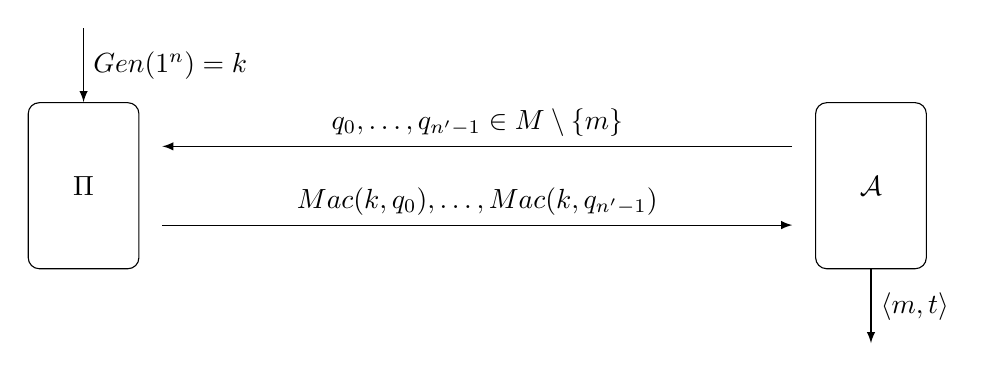
\begin{tikzpicture}[node distance=2cm,auto,>=latex]
\tikzset{
  player/.style={draw,shape=rectangle,rounded corners,minimum width=4em,minimum height=6em}
}
\node[player] (system) {$\Pi$};
\node[player] (adversary) at (10,0) {$\mathcal{A}$};
\draw[->] (9,0.5) -> node[above]{$q_0, \dots, q_{n'-1} \in M \setminus \{m\}$} (1,0.5);
\draw[->] (1,-0.5) -> node[above]{$Mac(k, q_0), \dots, Mac(k, q_{n'-1})$} (9,-0.5);
\draw[->] (0,2) -> node{$Gen(1^n) = k$} (system);
\draw[->] (adversary) -> node{$\langle m, t \rangle$} (10,-2);
\end{tikzpicture}
\end{center}

O desafio de $\mathcal{A}$ é produzir um par válido.
Chamamos o experimento de $MacForge_{\mathcal{A}, \Pi}$:
\begin{displaymath}
  MacForge_{\Pi, \mathcal{A}}(n) = Ver(k, m, t)
\end{displaymath}

Um sistema de autenticação de mensagem $\Pi = \langle Gen, Mac, Ver \rangle$ é {\em seguro contra falsificação} se para todo adversário eficiente $\mathcal{A}$ existe uma função desprezível $\varepsilon$ tal que:
\begin{displaymath}
  Pr[MacForge_{\Pi, \mathcal{A}}(n) = 1] \leq \frac{1}{2} + \varepsilon(n)
\end{displaymath}

O modelo de ataque considerado garante que um adversário não seja capaz de gerar código para uma mensagem nova, isto é, uma mensagem que não foi consultada.
Em alguns casos espeíficos queremos garantir também que o adversário não seja capaz de produzir outros tags válidos para uma mesma mensagem.
Este modelo de ataque é mais poderoso e chamaremos de {\em segurança forte contra falsificação}.

\subsection{CBC-MAC}
\label{sec:cbc-mac}

Agora que conhecemos o sistema de autenticação de mensagem e definimos uma noção de segurança, resta mostrar concretamente como construir tal sistema explicitando nossas suposições.
Começaremos com uma construção básica para uma mensagem de tamanho fixo baseada no modo CBC.
Vamos supor que $|m| = l.n$ em que $n$ é o tamanho do bloco de uma PRF $f$ e escreveremos $m = m_1 \dots m_l$ tal que $|m_i| = n$.
Temos então que:


\begin{itemize}
\item $Mac(k, m) := t_l$ em que:
  \begin{eqnarray*}
  t_0 & := & 0^n \\
  t_i & := & f_k(t_{i-1} \xor m_i) \textrm{ para i } = 1, \dots, l
  \end{eqnarray*}
 Além disso, $|m_i| = n$ e $f_k: \{0,1\}^n \to \{0,1\}^n$ é uma função pseudoaleatória.
\item $Ver(k, m, t) :=  \left\{
    \begin{array}{lcl}
      1 & \textrm{se} & t = Mac(k,m)\\
      0 & \textrm{c.c.} &\\
    \end{array}
    \right.$
  \end{itemize}

\begin{center}
\begin{tikzpicture}[node distance=2cm,auto,>=latex]
  \node (m1) at (0,0)  {$m_1$};
  \node (m2) at (2,0)  {$m_2$};
  \node (xor2) at (2,-2)  {$\xor$};
  \node (m3) at (4,0) {$m_3$};
  \node (xor3) at (4,-2)  {$\xor$};
  \node at (6,0) {\dots};
  \node at (6,-2) {\dots};
  \node (ml) at (8,0) {$m_l$};
  \node (xorl) at (8,-2)  {$\xor$};
  \node (t) at (10,-2)  {$t$};
  \draw[-] (m1) -> (0,-2);
  \draw[->] (0,-2) -> node[above]{$f_k$}(xor2);
  \draw[->] (m2) -> (xor2);
  \draw[->] (xor2) -> node[above]{$f_k$}(xor3);
  \draw[->] (m3) -> (xor3);
  \draw[->] (ml) ->  (xorl);
  \draw[->] (7,-2) -> node[above]{$f_k$}(xorl);
  \draw[->] (xorl) ->  (t);
\end{tikzpicture}
\end{center}


\begin{theorem}
  O sistema de autenticação $\Pi = \langle Gen, Mac, Ver \rangle$ como definido acima é seguro contra falsificação para mensagens de tamanho fixo $l.n$.
\end{theorem}

O sistema CBC-MAC é diferente do modo de operação CBC em dois aspectos essenciais: o MAC usa um bloco de $0$s onde o modo de operação usa um vetor inicial aleatório e o MAC expõe apenas o bloco final enquanto o modo de operação expõe cada um dos blocos cifrados.
É possível mostrar que ambas as diferenças são cruciais para garantir a segurança contra falsificação.

Para extender esta construção para mensagens de tamanho arbitrários temos duas opções para as quais há demonstração de segurança contra falsificação:
\begin{enumerate}
\item concatenar o tamanho da mensagem $|m|$ no começo da mensagem antes de produzir $t$ (concatenar no final não é seguro!).
\item gerar duas chaves independentes $k_1$ e $k_2$, usar a primeira no sistema apresentado acima e então computar $f_{k_2}(t)$ para gerar o código de autenticação.
\end{enumerate}

\section{Criptografia Autenticada}
\label{label}

O modelo de ameaças CPA assume que o adversário tem acesso a um oráculo $E_k$ que indica como mensagens escolhidas por ele podem seria criptografadas pelo sistema.
Com autenticação somos capaz de construir sistemas contra um modelo de ameaça ainda mais poderoso em que o adversário tem acesso a um oráculo em que ele pode consultar como determinadas cifras seriam decifradas.
Esse modelo de ameaças supõe um enorme poder por parte do adversário e é difícil encontrar exemplos práticos em que esse tipo de situação ocorra.
Ainda assim, é bastante interessante saber que é possível construir sistemas seguros contra este tipo de ameaça \cite{Naor90}.

Formalmente definimos um jogo da seguinte maneira:
\begin{enumerate}
\item O adversário $\mathcal{A}$ escolhe duas mensagens $m_0$ e $m_1$ com o mesmo tamanho ($|m_0| = |m_1|$) e envia para o sistema $\Pi$.
\item O sistema gera uma chave $k$ usando o algoritmo $Gen$ e sorteia aleatoriamente uma das mensagens para criptografar ($\Pi$ sorteia $b \leftarrow \{0, 1\}$ e criptografa $m_b$).
\item Durante todo o processo $\mathcal{A}$ possui acesso a um oráculo $E_k$ que ele pode usar para verificar como seria criptografadas qualquer mensagem $m$ e outro oráculo $D_k$ que ele pode usar para verificar como qualquer cifra $c$, exceto a cifra devolvida pelo sistema, seria decifrada.
\item A cifra produzida $E(k, m_b) = c$ e enviada de volta para o adversário.
\item O adversário $\mathcal{A}$ produz um bit $b' \in \{0,1\}$.
\end{enumerate}

\begin{center}
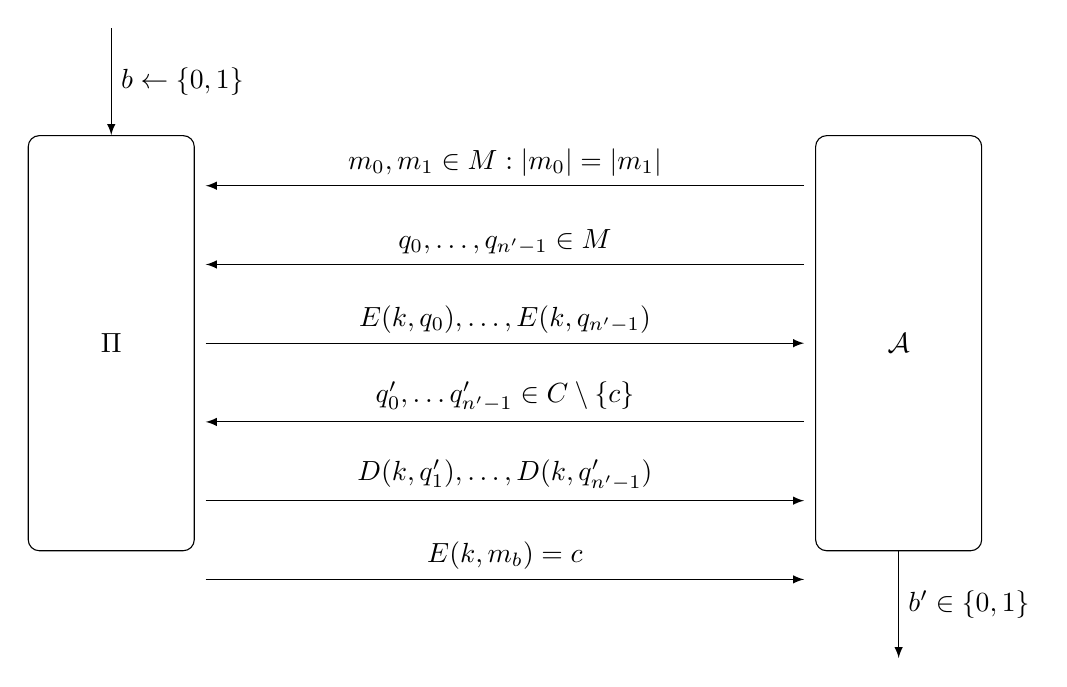
\begin{tikzpicture}[node distance=2cm,auto,>=latex]
\tikzset{
  player/.style={draw,shape=rectangle,rounded corners,minimum width=6em,minimum height=15em}
}
\node[player] (system) {$\Pi$};
\node[player] (adversary) at (10,0) {$\mathcal{A}$};
\draw[->] (8.8,2) -> node[above]{$m_0, m_1 \in M : |m_0| = |m_1|$} (1.2,2);
\draw[->] (8.8,1) -> node[above]{$q_0, \dots, q_{n'-1} \in M$} (1.2,1);
\draw[->] (1.2,0) -> node[above]{$E(k, q_0), \dots, E(k, q_{n'-1})$} (8.8,0);
\draw[->] (8.8,-1) -> node[above]{$q_0', \dots q_{n'-1}' \in C \setminus\{c\}$} (1.2,-1);
\draw[->] (1.2,-2) -> node[above]{$D(k,q_1'), \dots, D(k,q_{n'-1}')$} (8.8,-2);
\draw[->] (1.2,-3) -> node[above]{$E(k,m_b) = c$} (8.8,-3);
\draw[->] (0,4) -> node{$b \leftarrow \{0,1\}$} (system);
\draw[->] (adversary) -> node{$b' \in \{0,1\}$} (10,-4);
\end{tikzpicture}
\end{center}


O desafio de $\mathcal{A}$ é acertar qual das mensagens foi criptografada.
Como nos outros casos temos:
\begin{displaymath}
  PrivK^{cca}_{\Pi, \mathcal{A}}(n) = \left\{
    \begin{array}{lcl}
      1 & \textrm{se} & b = b'\\
      0 & \textrm{c.c.} &\\
    \end{array}
    \right.
\end{displaymath}

Dizemos que um sistema $\Pi = \langle Gen, E, D \rangle$ é seguro contra ataques do tipo {\em chosen ciphertext} (CCA) se para todo adversário eficiente $\mathcal{A}$ existe uma função desprezível $\varepsilon$ tal que:
\begin{displaymath}
  Pr[PrivK^{cca}_{\Pi, \mathcal{A}}(n) = 1] \leq \varepsilon(n)
\end{displaymath}

Note que os sistemas que não protegem a integridade da mensagem não são seguros contra CCA.
Por exemplo considere uma cifra de bloco no modo Ctr.
O adversário pode derrotar o jogo acima da seguinte forma:
\begin{enumerate}
\item $\mathcal{A}$ envia $m_0 = 0^n$ e $m_1 = 1^n$ para o sistema.
\item $\mathcal{A}$ recebe $c = E(k, m_b)$ e altera o primeiro bit de $c$ para produzir $c' \neq c$.
\item $\mathcal{A}$ consulta o oráculo $D_k(c')$ e verifica o resultado.
\item Se o resultado for $10^{n-1}$ o adversário devolve $0$, caso seja $01^{n-1}$ ele devolve $1$.
\end{enumerate}

Em um {\em sistema de criptografia autenticado} $\Pi$ o sistema ao descriptografar uma cifra $c$ deve acusar se ela não é válida devolvendo uma mensagem de erro.
Em nossa apresentação formal, $D(k,c) = \bot$ nestes casos.
Uma noção de segurança útil neste contexto é a capacidade de um sistema impedir que um adversário produza uma cifra válida.
Um sistema de criptografia $\Pi = \langle Gen, E, D \rangle$ é {\em seguro contra falsificação} se satisfizer essa noção de segurança.
(Omitiremos a formalização da definição de segurança contra falsificação que é análga a definição apresentada no final da Seção \ref{sec:mac}).
Por fim, chamaremos um sistema $\Pi$ de {\em sistema autenticado de criptografia} se $\Pi$ é seguro contra CCA e contra falsificação.

%Formalmente temos o seguinte jogo:
%\begin{enumerate}
%\item O sistema gera uma chave $k$ usando o algoritmo $Gen$.
%\item Durante todo o processo $\mathcal{A}$ possui acesso a um oráculo $E_k$ que ele pode usar para verificar como seria criptografadas qualquer mensagem $m$.
%\item O adversário $\mathcal{A}$ produz uma cifra $c$ tal que $E(k,m) \neq c$ para todos as consultas $m$ que o adversário fez ao oráculo.
%\end{enumerate}

%O desafio de $\mathcal{A}$ é produzir $c$ tal que $D(k,c) \neq \bot$:
%\begin{displaymath}
%  EncForge_{\Pi, \mathcal{A}}(n) = \left\{
%    \begin{array}{lcl}
%      1 & \textrm{se} & D(k,c) \neq \bot\\
%      0 & \textrm{c.c.} &\\
%    \end{array}
%    \right.
%\end{displaymath}

%Um sistema de criptografia $\Pi = \langle Gen, E, D \rangle$ é {\em seguro contra falsificação} se para todo adversário $\mathcal{A}$ eficiente temos que existe uma função desprezível $\varepsilon$ tal que:
%\begin{displaymath}
%  Pr[EncForge_{\mathcal{A},\Pi}(n) = 1] \leq \varepsilon(n)
%\end{displaymath}


Um sistema autenticado de criptografia é uma combinação de um esquema de criptografia com um sistema de autenticação.
Existem várias formas de combinar esses sistemas:
\begin{itemize}
\item {\em mac then encrypt}: produzimos um código de autenticação, juntamos esse código com a mensagem e criptografamos tudo.
\item {\em encrypt and mac}: enviamos separadamente a cifra e um código de autenticação da mensagem.
\item {\em encrypt then mac}: primeiro criptografamos e depois geramos o código da cifra.
\end{itemize}

Se nossa esquema de criptografia $\Pi_E = \langle Gen_E, E, D\rangle$ for seguro contra CPA e nosso sistema de autenticação $\Pi_M = \langle Gen_M, Mac, Ver \rangle$ for fortemente seguro contra falsificação, podemos demonstrar que o paradigma {\em encrypt then mac} é um {\em sistema autenticado de criptografia}, ou seja, é seguro contra CCA e contra falsificação.
Formalmente construimos o sistema $\langle Gen, E, D \rangle$ da seguinte forma:
\begin{itemize}
\item $Gen(1^n) := k = \langle k_E, k_M \rangle$ em que $Gen_E(1^n) := k_E$ e $Gen_M(1^n) := k_M$.
\item $E(k,m) := \langle c, t \rangle$ em que $E(k_E, m) := c$ e $Mac(k_M, c) := t$.
\item $D(k,c) := \left\{
    \begin{array}{lcl}
      D(k_E, c) & \textrm{se} & Ver(k_M, c, t)\\
      \bot & \textrm{c.c.} &\\
    \end{array}
    \right.$
\end{itemize}

O sistema acima gera chaves independentes $k_E$ e $k_M$ para os sistemas.
Isso não é apenas um detalhe, o uso da mesma chave de criptografia e autenticação pode causar sérios problemas de segurança.


\begin{example}
  Considere uma permutação pseudoaleatória $p$, escolha $r \leftarrow\{0,1\}^{n/2}$ e criptografe $m \in \{0,1\}^{n/2}$ da seguinte forma:
  \begin{displaymath}
    E(k,m) = p_k(m||r)
  \end{displaymath}
É possível mostrar que um sistema como esse é seguro contra CPA.

Agora considere um MAC que usa $p^{-1}$ para produzir o código:
\begin{displaymath}
  Mac(k,c) = p_k^{-1}(c).
\end{displaymath}
Também é possível mostrar que esse MAC é seguro contra falsificação.
Porém, quando aplicamos o pardigma {\em encrypt then mac} nesses sistemas temos que:
\begin{eqnarray*}
  E(k,m), Mac(k, E(k,m)) & = & p_k(m||r), p_k^{-1}(p_k(m||r))\\
                         & = & p_k(m||r), m||r
\end{eqnarray*}
Neste caso o código de autenticação vaza todo o conteúdo da mensagem!
\end{example}

\subsection{Comunicação Segura}
\label{sec:comunicacao-segura}

Um sistema autenticado de criptografia garante a confidencialidade, a integridade e a autenticidade na comunicação.
Existem, porém, outros tipos de ameaça que esse sistema não garante por si só:
\begin{itemize}
\item {\em ataque de reordenação:} um adversário pode embaralhar a ordem de mensagens seguras de forma a produzir um resultado malicioso.
\item {\em ataque de repetição:} um adversário pode encaminhar duas vezes uma mensma mensagem segura, por exemplo exigindo duas vezes um mesmo pagamento legítimo.
\item {\em ataque de reflexão:} um adversário pode enviar de volta para o próprio remetente uma mensagem como se fosse do destinatário.
\end{itemize}

Esses ataques tem soluções simples, mas que precisam ser tratadas quando produzimos um protocolo completo de comunicação segura.
Para resolver os dois primeiros problemas podemos manter um contador do número de mensagens $ctr_{AB}$ de $A$ para $B$ e $ctr_{BA}$ de $B$ para $A$.
O terceiro ataque pode ser resolvido inserindo um bit na mensagem que indique sua direção $b_{AB}$ é $1$ se a mensagem foi de $A$ para $B$ e $0$ caso contrário.
Outra possível solução para o terceiro problema é manter duas chaves independentes: uma $k_{AB}$ para a comunicação de $A$ para $B$ e outra $k_{BA}$ para a comunicação de $B$ para $A$.
Tanto o contador $ctr_{AB}$ quanto o bit de direção $b_{AB}$ devem ser concatenados a mensagem antes de criptografá-la.
No Capítulo \ref{cha:protocolos} veremos protocolos completos de segurança e voltaremos nesses detalhes.

Aqui encerramos os sistemas de criptografias que se baseiam no modelo simétrico.
Seguindo a abordagem moderna explicitamos as suposições necessária para provar a segurança de diversos sistemas de criptografia e autenticação.
O apêndice \ref{cha:owf} busca encontrar a suposição mínima que precisamos fazer para conseguir construir os sistemas que vimos até aqui, a saber, a existência de {\em funções de mão única}.
Além de servir como um bom resumo do que vimos até aqui, o apêndice procure justificar o porquê precisamos partir de determinadas suposições e não simplesmente provamos essas propriedades para cada sistema.

\section{Exercicios}
\label{sec:exercicios}


\begin{exercicio}
  Considere que o adversário sabe que a mensagem $m = 101010$ foi cifrada por uma cifra de fluxo e produziu $c = 110001$.
  Que sequencia de bits $c'$ ele precisa enviar para o destinatário para fazer com que ele ache que a mensagem original era $m' = 001011$?
\end{exercicio}


\begin{exercicio}
  Mostre que a função $encode$ que insere o tamanho da mensagem no começo e completa o último bloco com uma sequência de $0$s não admite prefixo.
\end{exercicio}

\begin{exercicio}
  Seja $f$ uma função pseudo-aleatória e considere o sistema $\Pi = \langle Gen, E, D \rangle$ uma cifra de bloco que aplica $f$ no modo contador.
  Suponha que Alice e Bob compartilham uma chave secreta $k$.
  Considere os seguintes cenários:
  \begin{enumerate}
  \item Alice enviar $E(k, m)$ para Bob que descriptografa usando a chave $k$
  \item Alice gera um checksum $H(m)$ da mensagem e envia $H(m)||m$ para Bob que pode verificar o checksum antes de ler a mensagem
  \end{enumerate}
  Algum desses cenários garante que a mensagem lida por Bob é idêntica a mensagem que foi enviada por Alice? Por que? Caso nenhum dos cenários garanta isso, descreva como poderíamos fazê-lo.
\end{exercicio}
